%Hello world! \textspanish{Me gusta el diseño gráfico}.
\begin{enumerate}
 \item 
 This is an example using a lot of mathematics an equations. 
 First, we show that we can create a simple equation like this:
 \begin{equation}
 \label{eq:elipse}
 \frac{x^{2}}{a^{2}} + \frac{y^{2}}{b^{2}} = 1
 \end{equation}
 And we can refer to it later in the text like this: the equation \eqref{eq:elipse} is an elipse. If we do not want to have it numbered we can say:
 \begin{equation}
 \nonumber
 \binom{n}{k} = \frac{n!}{k!(n-k)!} 
 \end{equation}
 And you can also embed equations into text for example: $\forall x \in \mathbb{R}$. 
 You can make links to an externam website like this: 
 To learn how to use the sumation and integrals you command you can check the \href{https://en.wikibooks.org/wiki/LaTeX/Mathematics#Sums_and_integrals}{wikibooks} 
 in or search for it in \url{www.google.com}.
 
 \item This is an example of an function with cases, like a \emph{pdf}.
 \begin{equation}
  \label{eq:pdf}
  f(y) =
  \begin{cases}
    \frac{1}{25} y & \quad \text{if } 0 \leq y < 5 \\
    \frac{2}{25} - \frac{1}{25} y & \quad \text{if } 5 \leq y < 10 \\
    0 & \quad \text{if } y < 0 \text{ or } y > 10
  \end{cases}
 \end{equation}
 An this is an example of an automatic sizing parenthesis:
 \begin{equation}
  \nonumber
  P\left(A=2\middle|\frac{A^2}{B}>4\right)
 \end{equation}
 An finally an integral in several steps: with $*$ you omit the numbers
\begin{align*}
P\left(X \leq 3 \right) &= \int_{0}^{3} \frac{1}{25} y \,\mathrm{d}y \\
     &= \left. \frac{1}{25} \cdot \frac{1}{2} \, y^{2} \right|_0^3 \\
     &= \frac{1}{25} \left( \frac{1}{2} \, 9 - \frac{1}{2} \, 0 \right) =
     \frac{1}{25} \cdot \frac{9}{2} = \frac{9}{50} \approx 0.18 
\end{align*}

 \item This is an example of how to place figures. The most basic way is to place a figure as a center paragraph with his caption.
 
 
\begin{figure}[htb]
  \centering
  \label{fig:one}
  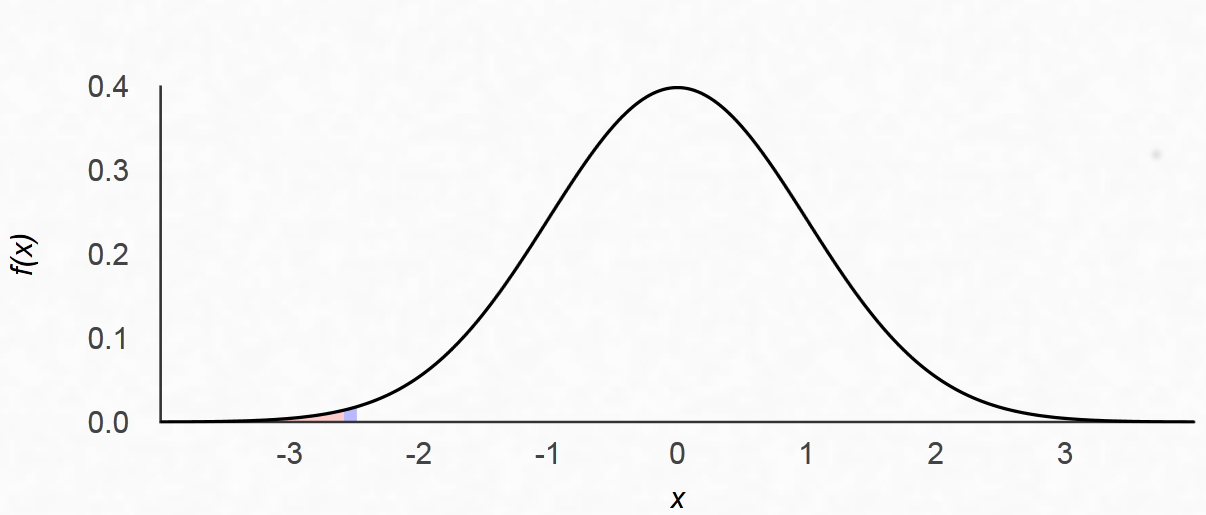
\includegraphics[width=0.5\textwidth]{img/normal}
  \caption{Area corresponding to $z$-value of -2.5298.}
\end{figure}

But it also could be that a figure is composed of several subfigures each with his caption and an extra caption for the whole group. See Figure~\ref{fig:two} or refer to subfigure like this. See Figure~\ref{fig:2b}.

\begin{figure}[htp]
  \centering
  \begin{subfigure}[b]{0.3\textwidth}
    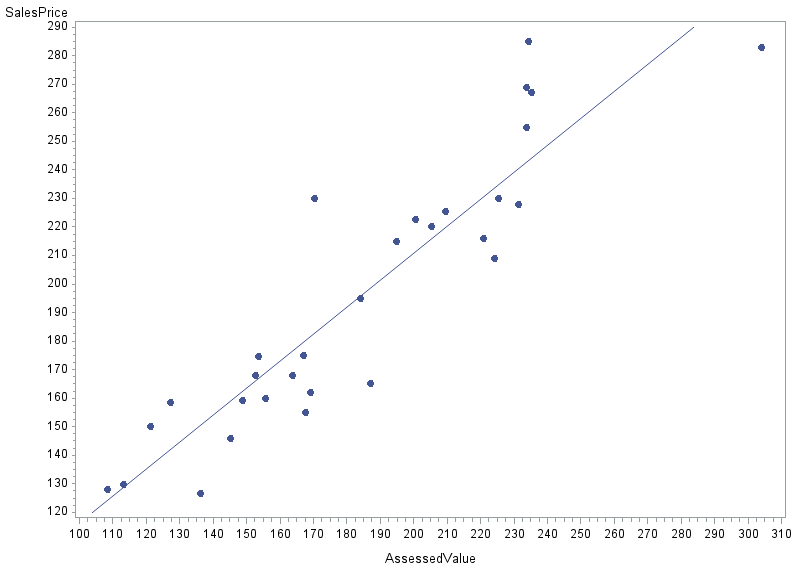
\includegraphics[width=\textwidth]{img/scatter}
    \caption{Scatter plot Assessed value v.s. sales price.}
  \label{fig:2a}
  \end{subfigure}
    ~
  \begin{subfigure}[b]{0.3\textwidth}
    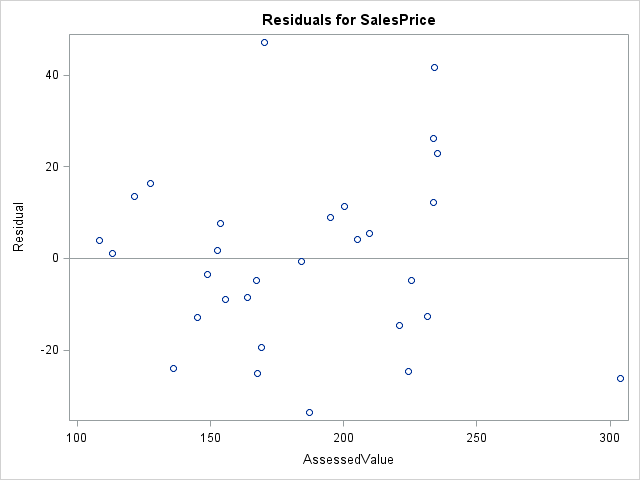
\includegraphics[width=\textwidth]{img/residuals}
    \caption{Residuals vs assesed value.}
    \label{fig:2b}
  \end{subfigure}
  ~
  \begin{subfigure}[b]{0.3\textwidth}
    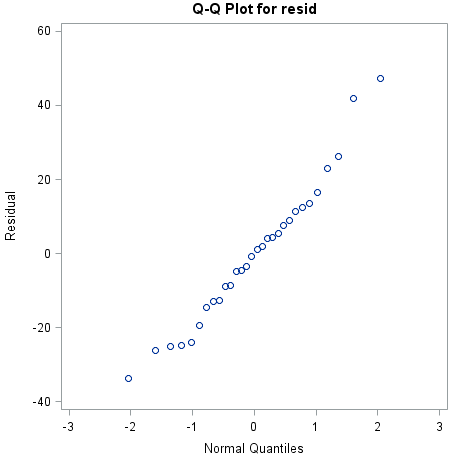
\includegraphics[width=\textwidth]{img/qqplot}
    \caption{Normal quantile plot of the residuals.}
    \label{fig:2c}
  \end{subfigure}
    
  \caption{Plots of an imaginary exercise, lets call it $X$.}
  \label{fig:two}
\end{figure}

\item This is an example of how to cite a book. This exercise was taken from~\cite{Devore2012}. And finally this is an example of a very nice table: Table \ref{tab:exey}

\begin{table}[htb]
  \begin{center}
    \begin{tabular}{l | r r r r r}
      \toprule
      Source & \textbf{DF} & \textbf{SS} & \textbf{MS} & \textbf{F} & \textbf{P-value} \\
      \midrule
      \textbf{Model} & 2 & 0.00318564 & 0.00159282 & 7.72 & 0.0014 \\
      \textbf{Error} & 42 & 0.00866760 & 0.00020637 &  & \\
      \midrule
      \textbf{Total} & 44 & 0.01185324 &   &  & \\
      \bottomrule
    \end{tabular}
  \end{center}
\caption{Anova table for exercise $y$}
\label{tab:exey}
\end{table}

\item Lets look at how to write an algorith using pseudo code. See the algorithm~\ref{alg:euclid}. The while ends in line~\ref{euclidendwhile}. The information comes from this part of the \href{https://en.wikibooks.org/wiki/LaTeX/Algorithms#Typesetting_using_the_algorithmicx_package}{wikibook} and from this \href{https://tex.stackexchange.com/questions/229355/algorithm-algorithmic-algorithmicx-algorithm2e-algpseudocode-confused}{post}.

\begin{algorithm}
  \caption{Euclid's algorithm}
  \label{alg:euclid}
  \begin{algorithmic}[1] % The number tells where the line numbering should start 0 for no number
    \Procedure{Euclid}{$a,b$} \Comment{The g.c.d. of $a$ and $b$}
      \State $r\gets a \bmod b$
      \While{$r\not=0$} \Comment{We have the answer if $r = 0$}
        \State $a \gets b$
        \State $b \gets r$
        \State $r \gets a \bmod b$
      \EndWhile\label{euclidendwhile}
      \State \textbf{return} $b$\Comment{$gcd = b$}
    \EndProcedure
  \end{algorithmic}
\end{algorithm}

\item We are going to implement the algorithm in C++ language. And see if we can put the source code. This is an example of minted:
\begin{minted}{c}
int main() {
  printf("hello, world");
  return 0;
}
\end{minted}

This is another example; this time on the \emph{R language}

\begin{minted}{R}

 A <- matrix(c(0.15, 0.01, 0,
               0.14, 0.36, 0.07,
               0.15, 0.13, 0.3), ncol = 3, byrow = TRUE)
 I = diag(nrow = nrow(A))

 I%*%A
\end{minted}

This is another example of inlined code: \mintinline{python}{print(x**2)} lets see how it looks. Finally, lets try to input another file: See Listing \ref{lst:example}. I took a lot of help form \href{https://tex.stackexchange.com/questions/252263/alignment-of-minted-line-numbers}{here} and \href{https://www.overleaf.com/learn/latex/Code_Highlighting_with_minted}{Overleaf help}.
\begin{listing}[H]
\inputminted[
xleftmargin=1cm,  %without this option line number goes wrong
%frame=lines,
framesep=0.5cm,
baselinestretch=1.2,
%fontsize=\footnotesize,
linenos,
firstline=54, %If yu omit this two the whole file is pulled 
lastline=68
]{cpp}{src/GccTest.cpp}
\caption{My buggy implementation of insertion sort. (Do not use)}
\label{lst:example}
\end{listing}

\end{enumerate}
